\begin{lstlisting}[language=Python]
att = (A_K.cpu().detach().numpy()@b.T ).T @ (A_Q.cpu().detach().numpy()@b.T )
att = att.reshape(1,1,32,32)
att = torch.tensor(att)
head_view((att,), tokens)
\end{lstlisting}


\vspace{0.5em}
\begin{figure}[h]
    \centering
    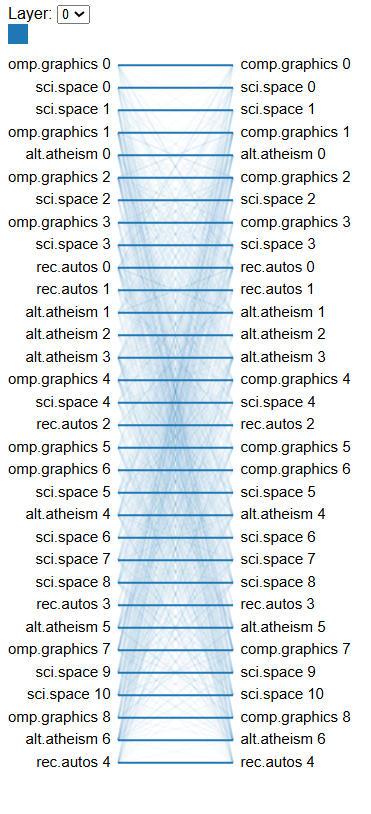
\includegraphics[width=0.45\textwidth]{../figures/4/attention_begin.png}
    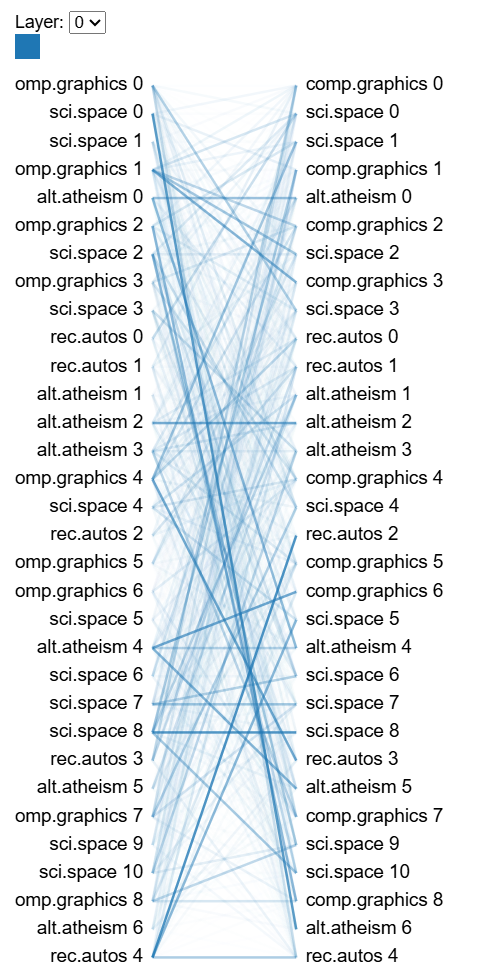
\includegraphics[width=0.45\textwidth]{../figures/4/attention_learned.png}
    \caption{Comparação entre a visualização de atenção inicial (TF-IDF) e após o treinamento (atenção aprendida)}
    \label{fig:attention_comparison}
\end{figure}

\vspace{0.5em}
\noindent O resultado do presente head\_view apresenta relações entre amostras da mesma classe mais fortes que o head\_view do item (a), indicando o impacto do treinamento na definição da similaridade.
\noindent A comparação entre as visualizações mostra que a rede aprendeu a criar representações que aumentam a similaridade entre artigos da mesma categoria, demonstrando que o mecanismo de atenção pode aprender padrões mais sofisticados que a simples sobreposição de termos.
\noindent Isso implica em uma matriz mais esparsa e focada, onde as relações entre amostras da mesma classe são ressaltadas.

